\chapter{Methodology}

This chapter explains how the framework was designed, how the metrics were formalised, and how the implementation and empirical evidence were evaluated.

\section{Research Design and Approach}

This research uses design science to create and evaluate an artefact: a multidimensional intrinsic evaluation framework for RDF-based event-centric knowledge graphs. This approach is appropriate because the primary contribution is the formalised framework. The accompanying software executes its definitions and repeats the same calculations on different RDF inputs \citep{hevner2004}.

The study proceeded in three stages. First, a targeted literature synthesis identified candidate quality concerns and possible ways to measure them. Second, the selected calculations were formalised, implemented, and checked with small RDF fixtures whose expected values could be calculated by hand. Third, the empirical evaluation examined whether the calculations responded to known changes in three controlled datasets, how four general RDF/KG tools responded to the same inputs, and whether the evaluator could run on the published OEKG event layer and public ChronoGrapher graph artefacts. The controlled test is called a sensitivity test because it checks whether a result changes when a property that it measures is deliberately changed.

Development within these stages was iterative, but it did not follow a fixed number of identical experimental cycles. Here, \emph{refinement} means correcting a metric definition, population rule, or implementation after a small fixture exposed an error. These corrections were completed before the accepted experiments were run. The controlled datasets were then regenerated from fixed profiles, the ChronoGrapher files were converted to N-Triples, and seven invalid literal escapes in the OEKG event layer were repaired. All accepted D1--D3, comparator, ChronoGrapher, and OEKG results were produced with the same frozen corrected evaluator snapshot. The repository verification script confirms that the current evaluator source and every accepted result still match that snapshot.

The framework, rather than the software alone, remains the central contribution. The implementation operationalises the framework and tests whether its definitions can be executed repeatably on controlled and public RDF event data.

Figure \ref{fig:methodology_pipeline} summarises the resulting evaluation and verification workflow.

\begin{figure}[H]
\centering
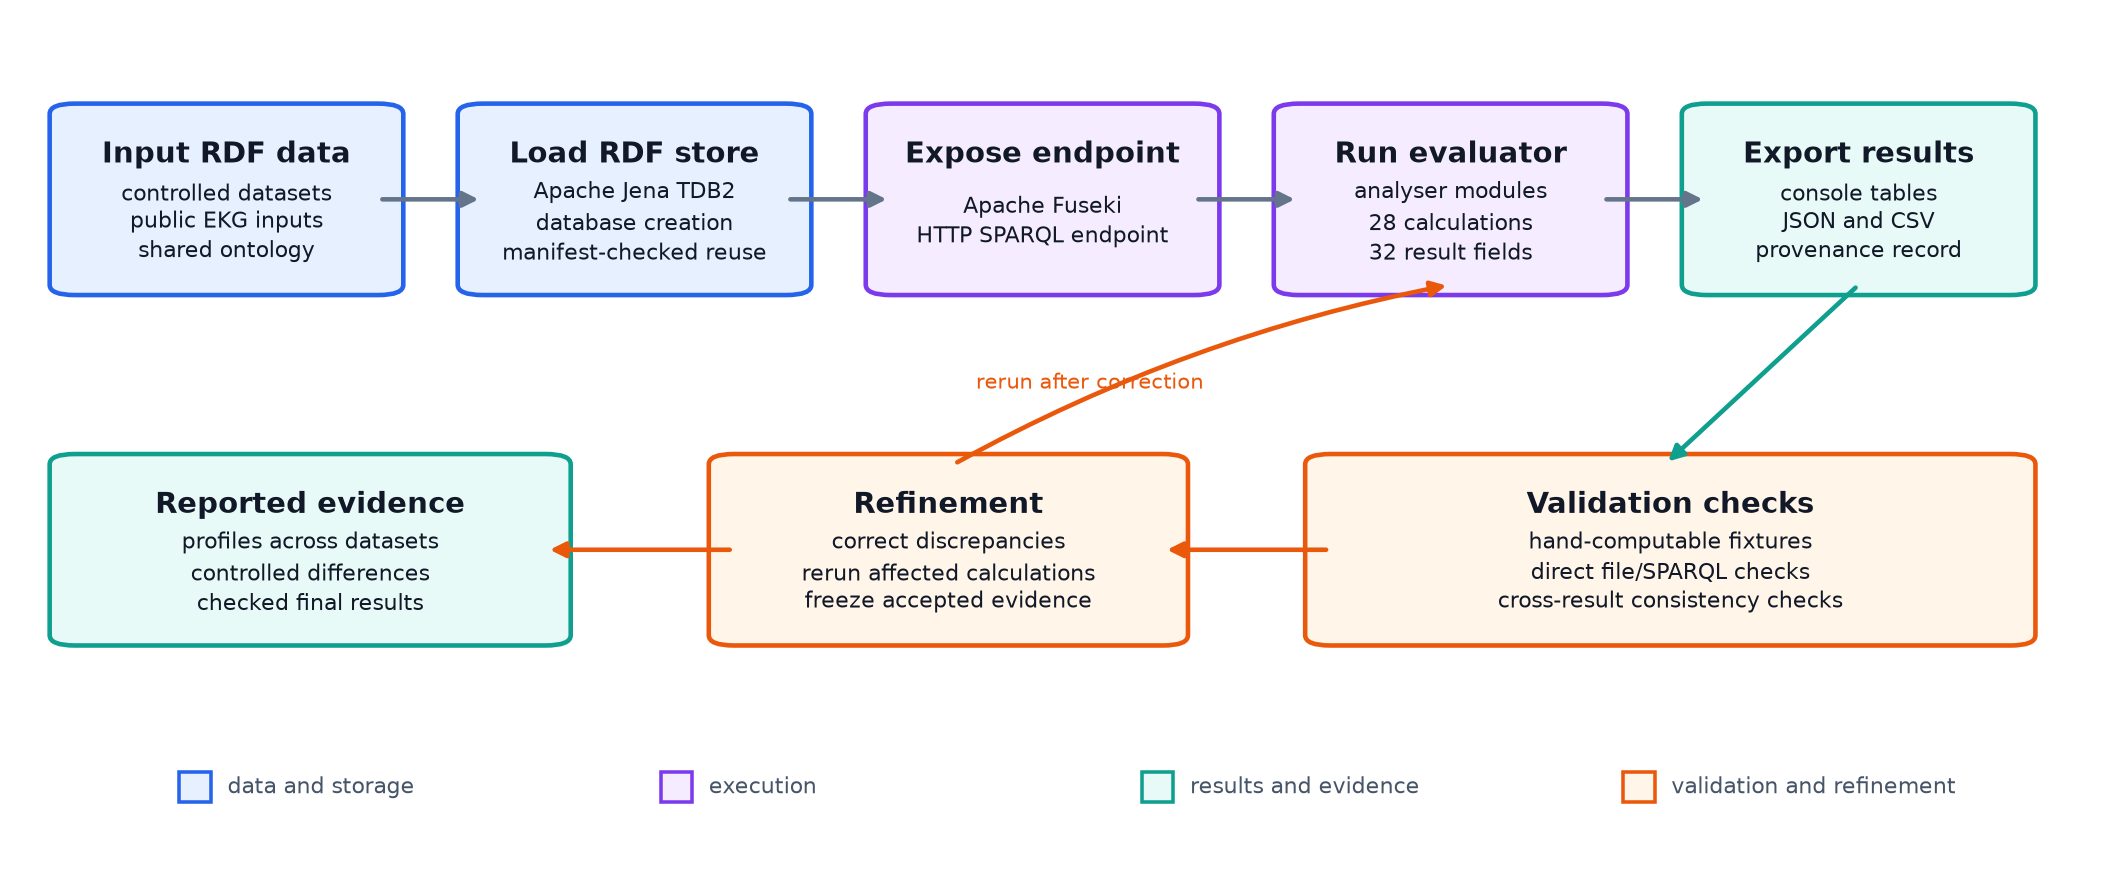
\includegraphics[width=\textwidth]{evaluation_pipeline_diagram.png}
\caption{Evaluation workflow. Refinement refers to corrections made after fixture checks and before the accepted experiments were frozen.}
\label{fig:methodology_pipeline}
\end{figure}

\section{Literature Selection and Framework Derivation}

The framework was informed by a structured, targeted review of EKG evaluation, temporal evaluation, general KG quality, and RDF validation. The review sought candidate quality concerns, existing formulae, formal rules, and evaluation procedures that could be used or adapted for RDF-based EKGs.

The review covered work from ACM Digital Library, IEEE Xplore, Scopus, Web of Science, Google Scholar, ACL Anthology, and Semantic Scholar. The search queries covered literature available up to May 2026 and used the following Boolean combinations:

\begin{itemize}
    \item (``event-centric knowledge graph'' OR ``event knowledge graph'' OR EventKG OR OEKG OR ASER) AND (evaluation OR quality OR assessment OR validation)
    \item (``knowledge graph'' AND (quality OR completeness OR consistency OR conformance OR coverage) AND (metric* OR framework))
    \item (temporal AND (``event knowledge graph'' OR ``knowledge graph'') AND (evaluation OR ``temporal consistency'' OR granularity OR density))
    \item (``schema conformance'' OR ``RDF validation'' OR ``type consistency'' OR ``RDF Schema'') AND (``knowledge graph'' OR RDF)
    \item (``event-centric question answering'' OR Event-QA OR KGrEaT OR ``downstream task'') AND (``knowledge graph'' OR benchmark OR evaluation)
\end{itemize}

Screening proceeded in three stages. First, titles and abstracts were screened for work on event-centric representation, KG quality, temporal evaluation, RDF/schema validation, or event-centric downstream evaluation. Second, full texts were retained when they provided reusable dimensions, formulae, constraints, validation procedures, or benchmark designs. Third, backward and forward snowballing was applied to seed papers and standards. Exact per-database hit counts and a deduplicated screening log were not retained. Relevant work may therefore have been missed, and this review cannot support the absolute claim that no other framework exists. The narrower claim used in this thesis is that none of the sources and tools reviewed up to May 2026 operationalised all nine selected intrinsic dimensions for RDF-based EKGs. Table \ref{tab:key_ekg_eval_papers} identifies the main sources used, and Table \ref{tab:literature_to_metrics_mapping} shows how their findings informed the final metric groups.

Studies were included when they met at least one of the following criteria: (1) direct relevance to event-centric knowledge graphs or event graphs, (2) contribution of a transferable KG evaluation dimension or metric, (3) contribution of formal validation rules applicable to RDF graphs, or (4) contribution of a benchmark or validation method relevant to EKG assessment. Studies were excluded when they focused only on event extraction or graph construction without reusable evaluation content, when their evaluation logic was too domain-specific to transfer to RDF/EKG settings, or when the work was a duplicate preprint/final-publication pair. Original papers and official standards were prioritised over secondary summaries when both were available.

The included literature fell into three groups:
\begin{itemize}
    \item \textbf{Direct EKG sources} such as EventKG, OEKG, ASER, NewsReader-style EKGs, and Event-QA identified quality concerns that arise in event-centric graph practice, including temporal coverage, contextual completeness, source integration, external linking, and downstream event-centric querying \citep{eventkg2018,oekg2023,aser2019,newsreader2016,eventqa2020}.
    \item \textbf{Foundational event and temporal sources} such as SEM, TimeML, temporal evaluation work, and temporal information evaluation frameworks identified event-specific representational requirements such as events, actors, places, time, temporal anchoring, granularity, and temporal consistency \citep{sem2011,timeml2003,tempeval2011,tieval2023}.
    \item \textbf{General KG quality and RDF validation sources} such as RDF Schema, Luzzu, test-driven linked data quality assessment, KGrEaT, and scalable KG auditing contributed reusable principles for schema-aware validation, modular metrics, intrinsic/extrinsic evaluation boundaries, and scalable validation \citep{rdfs2014,luzzu2016,testdriven2014,kgreat2023,efficienteval2019}.
\end{itemize}

\begin{table}[htbp]
\centering
\scriptsize
\caption{Key sources used to derive EKG evaluation dimensions and metrics. The use codes indicate whether a source was directly relevant to EKG evaluation (R), contributed quality dimensions (D), or contributed concrete metrics, operational rules, or validation procedures (M).}
\label{tab:key_ekg_eval_papers}
\setlength{\tabcolsep}{3pt}
\begin{tabularx}{\textwidth}{>{\raggedright\arraybackslash}p{2.4cm}>{\raggedright\arraybackslash}p{1.9cm}>{\raggedright\arraybackslash}p{0.7cm}>{\raggedright\arraybackslash}p{2.0cm}X>{\raggedright\arraybackslash}p{0.8cm}}
\toprule
\textbf{Source} & \textbf{Authors} & \textbf{Year} & \textbf{Primary focus} & \textbf{Contribution to framework} & \textbf{Use} \\
\midrule
Simple Event Model \citep{sem2011} & van Hage et al. & 2011 & Core event representation & Defines events, actors, places, and time as core event variables; motivates completeness, contextual grounding, and temporal-property checks. & D, M \\
TimeML \citep{timeml2003} & Pustejovsky et al. & 2005 & Temporal and event markup & Motivates temporal grounding, event ordering, and reasoning over underspecified time expressions. & D, M \\
Temporal Evaluation \citep{tempeval2011} & UzZaman and Allen & 2011 & Temporal evaluation & Motivates consistency-aware temporal evaluation beyond exact edge matching. & D, M \\
EventKG \citep{eventkg2018} & Gottschalk and Demidova & 2018 & Multilingual EKG & Direct EKG source; motivates temporal coverage, contextual completeness, source integration, and external-link coverage. & R, D, M \\
NewsReader EKGs \citep{newsreader2016} & Rospocher et al. & 2016 & News-based EKG construction & Shows reliance on sampled human judgement where full gold standards are unavailable; motivates scalable intrinsic metrics. & R, D \\
ASER \citep{aser2019} & Zhang et al. & 2020 & Eventuality KG & Contributes event-graph validation patterns and highlights the intrinsic/extrinsic evaluation distinction. & R, D, M \\
OEKG \citep{oekg2023} & Gottschalk et al. & 2021 & Integrated open EKG & Motivates common-schema assessment, multilingual integration, and use-case-oriented utility. & R, D \\
RDF Schema \citep{rdfs2014} & W3C & 2014 & RDF vocabulary semantics & Provides class, subclass, domain, range, and datatype semantics used to motivate profile and type-consistency checks. & M \\
Luzzu \citep{luzzu2016} & Debattista et al. & 2016 & Linked data quality & Contributes multidimensional quality design, metric modularity, and automation principles. & D, M \\
Event-QA \citep{eventqa2020} & Souza Costa et al. & 2020 & Event-centric QA benchmark & Motivates future extrinsic validation and task-utility linkage. & R, D \\
ChronoGrapher \citep{chronographer2023} & Blin et al. & 2025 & EKG construction and QA & Provides a public SEM-based event-graph construction case with construction-accuracy and downstream QA evaluation; motivates comparison between task/evaluation utility and intrinsic graph-quality profiling. & R, D \\
\texttt{tieval} \citep{tieval2023} & Sousa et al. & 2023 & Temporal IE evaluation & Highlights cross-dataset incompatibility in temporal evaluation and supports temporal-awareness-oriented metric design. & D, M \\
KGrEaT \citep{kgreat2023} & Heist et al. & 2023 & Downstream KG utility & Shows that correctness and completeness alone do not capture task utility; motivates explicit intrinsic/extrinsic scope boundaries. & D \\
Efficient KG accuracy evaluation \citep{efficienteval2019} & Gao et al. & 2019 & Scalable KG auditing & Contributes sampling-based validation logic for future human-in-the-loop auditing when full graph annotation is infeasible. & M \\
\bottomrule
\end{tabularx}
\end{table}

For each included source, three kinds of information were recorded: quality concerns treated as important for event-centric or temporal graphs, formulae or formal rules that could be applied to RDF data, and gaps showing where existing evaluation covered only part of the graph. Candidate dimensions were retained when they were relevant to event representation, could be measured through RDF/SPARQL or graph analysis, and produced a result that could be traced to a specific graph property.

\begin{table}[htbp]
\centering
\scriptsize
\caption{Mapping from literature findings to candidate dimensions and final metric groups. The table shows how evidence from event modelling, temporal evaluation, RDF validation, and KG quality literature was translated into the framework's implemented metric categories.}
\label{tab:literature_to_metrics_mapping}
\setlength{\tabcolsep}{3pt}
\begin{tabularx}{\textwidth}{>{\raggedright\arraybackslash}p{4.0cm}>{\raggedright\arraybackslash}p{3.0cm}X}
\toprule
\textbf{Literature finding} & \textbf{Candidate dimension} & \textbf{Final metrics operationalised in the framework} \\
\midrule
SEM treats event, actor, place, and time as the core variables of event representation. & Completeness, coverage, and entity richness & Label coverage, date coverage, location coverage, population completeness, average properties per event, sparse entities. \\
TimeML and temporal evaluation work emphasise temporal anchoring, ordering, granularity, and logical consistency. & Temporal consistency & ISO 8601 compliance, temporal coverage, granularity, temporal span, average events per decade, and interval consistency. \\
EventKG and OEKG show that event graphs depend on temporal/spatial/contextual coverage and external source integration. & External mapping coverage; contextual completeness & External link rate, Wikidata coverage, DBpedia coverage, completeness-related coverage metrics. \\
RDF Schema and RDF validation practice provide datatype, class, domain, range, and vocabulary-alignment principles. & Minimal event-profile alignment; closed-profile type alignment & Label and temporal coverage, minimum label/time/place profile, non-standard property diagnostic, and evidence-weighted type alignment. \\
Luzzu and linked data quality work show that quality is multidimensional and should be operationalised through modular, automatable metrics. & Structural and usage dimensions & Number of connected components, giant component ratio, clustering, density, average degree, predicate entropy, and HHI concentration. \\
Multi-source event integration creates duplicate risk and label redundancy. & Redundancy and duplication & Duplication rate, label uniqueness rate, fuzzy duplicate pairs. \\
Direct EKG papers often validate only narrow slices of quality, leaving graph-level quality fragmented. & Comprehensive synthesis across dimensions & Final nine-dimension framework rather than a single precision/recall or task-only evaluation. \\
Event-QA and KGrEaT show the importance of downstream usefulness, but not all intrinsic quality dimensions can be reduced to a single task benchmark. & Future extrinsic validation layer & Kept outside the implemented intrinsic framework; used to justify future task-based validation. \\
Scalable KG auditing work shows that exhaustive human validation is costly for large KGs. & Scalable validation procedure & Future extension through stratified or sampled human auditing rather than mandatory full-graph manual annotation. \\
\bottomrule
\end{tabularx}
\end{table}

The review served two concrete purposes. Table \ref{tab:key_ekg_eval_papers} identifies the sources from which event requirements, quality concerns, formulae, or validation procedures were taken. Table \ref{tab:literature_to_metrics_mapping} then links those findings to candidate dimensions and to the calculations implemented in this thesis. The review therefore synthesised existing work to identify what might be measured; it did not treat every concern in the literature as a completed framework dimension. The core framework retained concerns that were relevant to event representation and could be computed from RDF data. Downstream task utility and sampled factual auditing require different evidence and remain extensions.

Every calculation named in the final column of Table \ref{tab:literature_to_metrics_mapping} was checked against the definitive 32-field inventory in Appendix \ref{app:core_metric_inventory}. The table uses shorter descriptive names, while the appendix gives the exact result-field names, formulae, and implementation paths.

\section{Framework Design Process}

This section explains how the candidate concerns in Table \ref{tab:literature_to_metrics_mapping} were reduced to the final dimensions and how those dimensions are presented in the framework.

\subsection{Dimension Identification}

Table \ref{tab:literature_to_metrics_mapping} is the bridge between the review and the framework. Its first column states a finding from prior work, its second column identifies the quality concern raised by that finding, and its third column names the calculations used to examine that concern. Candidate concerns were retained when they were relevant to RDF event representation, could be measured automatically from the available graph evidence, and produced a result that could be traced to a specific graph property. This selection means that the framework covers selected computable intrinsic concerns; it does not claim that non-computable concerns such as factual truth or task suitability are irrelevant.

For example, temporal coverage was retained because SEM and EKG work treat temporal grounding as part of event representation and it can be measured by counting distinct events with a begin or end timestamp. External mapping coverage was retained because integrated EKGs use explicit links to connect event resources with external knowledge bases. Redundancy was retained because integration can produce repeated event descriptions. These examples show how Table \ref{tab:literature_to_metrics_mapping} informed selection without repeating the literature review itself.

The nine core dimensions are graph connectivity and structure, redundancy and duplication, temporal consistency, minimal event-profile alignment, completeness, closed-profile type alignment, entity richness, external mapping coverage, and predicate usage. For presentation, these nine dimensions are grouped into five conceptual families: structural integrity, temporal quality, semantic/profile quality, completeness and richness, and external/usage quality.

Structural integrity combines graph connectivity and redundancy checks because both describe coherence, fragmentation, or duplication risk. Temporal quality focuses on temporal representation and ordering. Semantic/profile quality groups minimum-profile and explicit type-alignment checks, since both assess fit to declared RDF expectations without claiming open-world logical invalidity. Completeness and richness bring together event-property completeness and event description breadth, while external/usage quality covers explicit mapping coverage and predicate distribution. These groupings are presentational; the implementation still reports the nine dimensions separately.

Figure \ref{fig:framework_dimensions} serves a different purpose from Table \ref{tab:literature_to_metrics_mapping}. The table documents where the candidate concerns came from; the figure groups the nine final dimensions into five presentational families. Neither combines the dimensions into one score.

\begin{figure}[htbp]
\centering
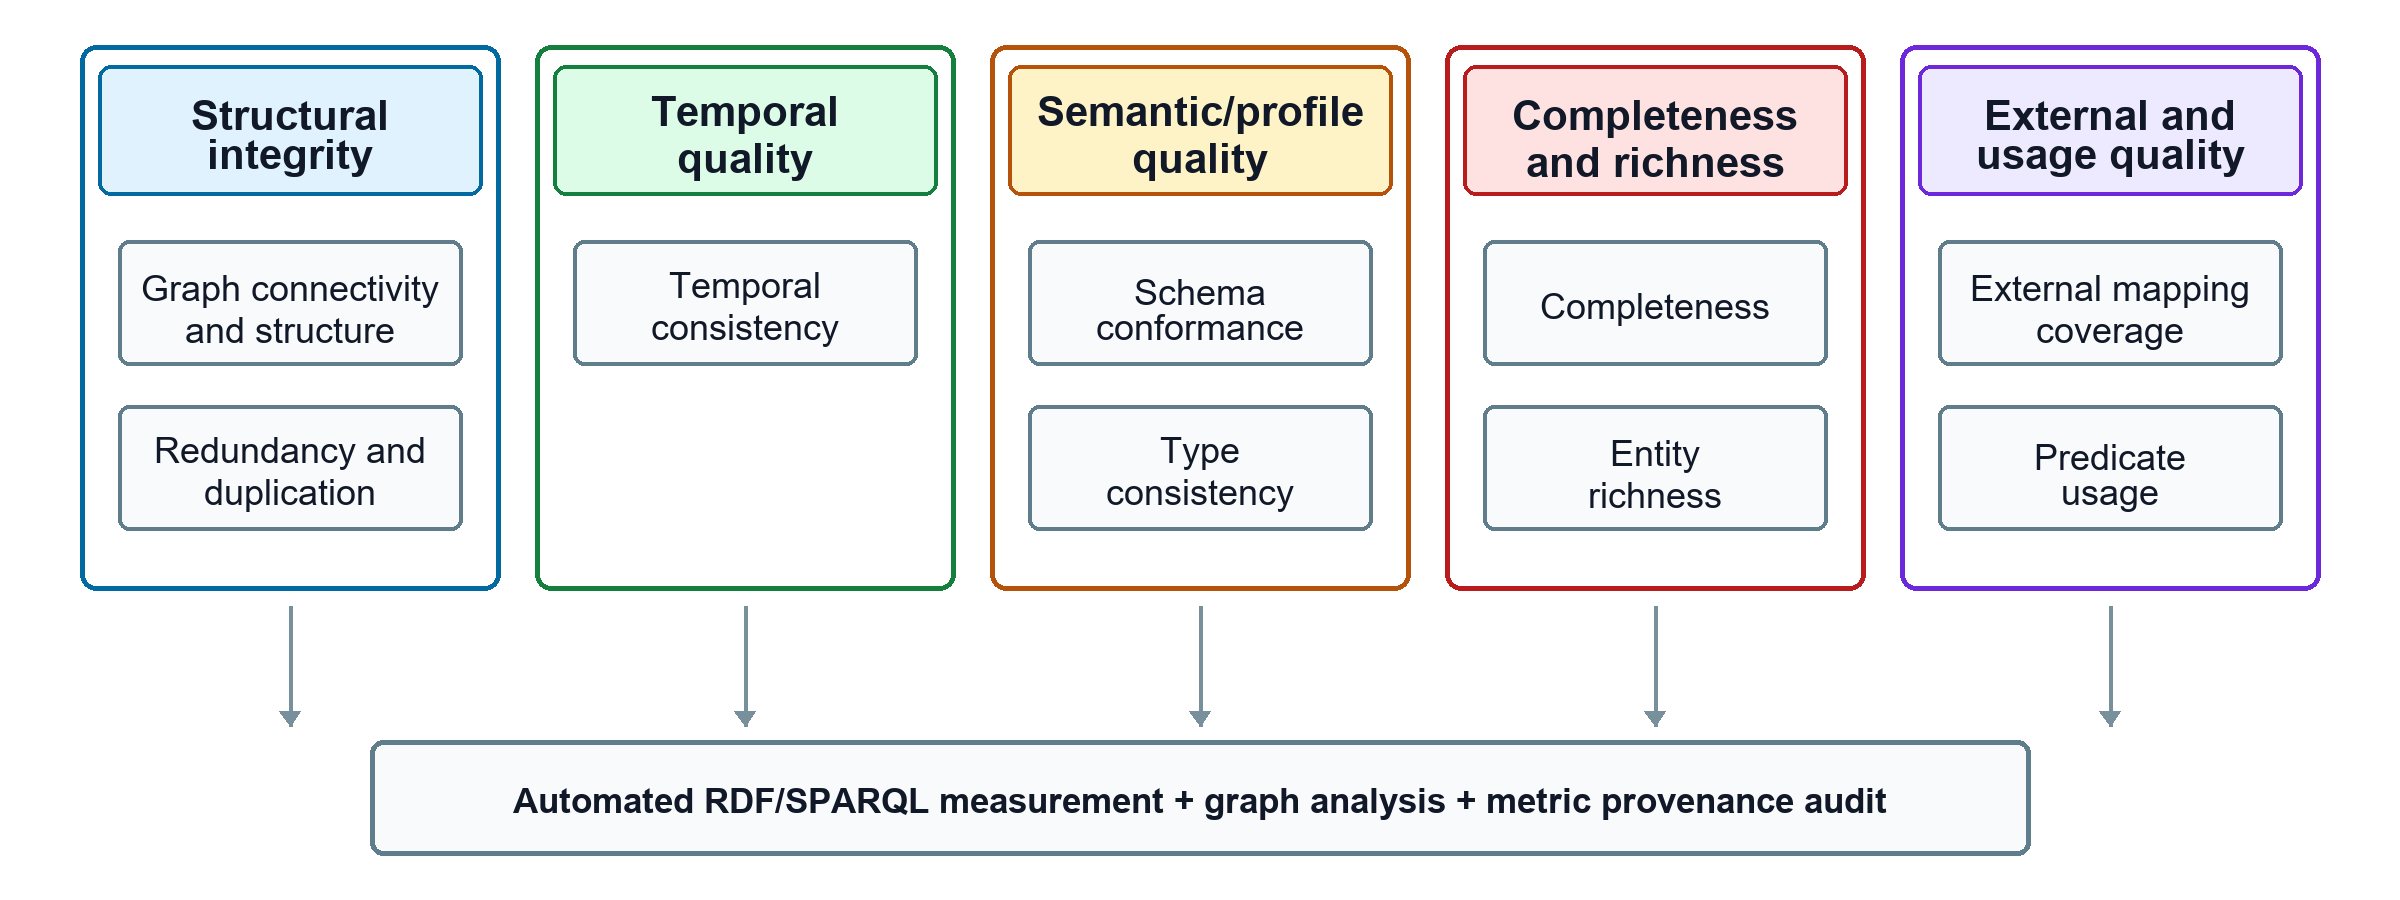
\includegraphics[width=\textwidth]{framework_dimensions_diagram.png}
\caption{Conceptual grouping of the nine core EKG quality dimensions into five presentational families. The framework reports the nine dimensions individually, while the figure shows how related dimensions form a multidimensional quality profile.}
\label{fig:framework_dimensions}
\end{figure}

\subsection{Design Principles}

Four principles guided framework design: automation, standards alignment, modularity, and transparency. Automation means that the calculations can be run from RDF data without manual annotation. Standards alignment means that the implementation follows RDF data structures, RDFS and OWL vocabulary semantics, SPARQL query semantics, XML Schema datatypes, and the SEM and OWL-Time terms used by the declared profile. This does not mean that every input graph conforms to one universal EKG standard.

Modularity means that each evaluation dimension is defined as a separable part of the framework, so users can inspect, run, or extend dimensions independently. Transparency is supported by documenting graph projection decisions, normalisation algorithms, sampling strategies, metric provenance, and the boundary between metrics taken from established formulas and metrics formalised in this thesis.

\section{Metric Development and Formalisation}

This section explains how the framework dimensions were turned into calculations. An \emph{adopted} metric uses an established formula without changing its mathematical definition. An \emph{adapted} metric applies an established quality principle to the direct-event population and predicates used in this study. A metric \emph{formalised in this thesis} addresses a concern found in the literature for which no directly reusable RDF-EKG formula was identified; its exact denominator, threshold, or aggregation rule was therefore specified here. Appendix \ref{app:core_metric_inventory} records the classification and source basis of every registered result field.

\subsection{Metric Operationalisation}

Each dimension was operationalised in four steps. The quality concern was first stated in words. Its calculation was then adopted, adapted, or formalised in this thesis. Next, the formula and empty-case rule were specified. Finally, the calculation was implemented as a SPARQL query, file scan, or graph algorithm. Small RDF fixtures with values calculated by hand were used to check the implementation. Additional consistency checks tested relationships that must hold between results, such as covered events plus missing events equalling the event population.

The implementation returns 32 named result fields across the nine dimensions. These fields represent 28 distinct calculations: four fields repeat an existing calculation under another module so that each module can return a complete local report. The implementation also returns 73 supporting fields, such as numerators, denominators, sample sizes, status messages, and per-property breakdowns. Supporting fields explain how a result was obtained but are not additional metrics.

Table \ref{tab:metrics_summary} shows how the 32 registered result fields are distributed across the nine dimensions. Appendix \ref{app:core_metric_inventory} assigns them the identifiers M01--M32 and records each field's output path, formula, implementation, empty-case rule, and provenance. These identifiers are labels used for auditing; they are not scores or separate claims of quality.

\begin{table}[H]
\centering
\caption{Distribution of the 32 registered result fields across the nine EKG evaluation dimensions. Four fields are aliases, so the table represents 28 distinct calculations.}
\label{tab:metrics_summary}
\begin{tabular}{lc}
\toprule
\textbf{Dimension} & \textbf{Registered result fields} \\
\midrule
Graph Connectivity \& Structure & 6 \\
Redundancy \& Duplication & 3 \\
Temporal Consistency & 6 \\
Minimal Event-Profile Alignment & 4 \\
Completeness & 5 \\
Type Consistency & 1 \\
Entity Richness & 2 \\
External Mapping Coverage & 3 \\
Predicate Usage & 2 \\
\midrule
\textbf{Total} & \textbf{32} \\
\bottomrule
\end{tabular}
\end{table}

The 32 fields include four aliases. M16 and M22 both report label coverage. M12, M17, and M23 all report temporal coverage, creating two repeated fields. M18 and M21 both report the same label--time--place profile rate. The aliases are retained because the temporal, profile, and completeness modules each need to show the relevant value in their own output. They are labelled as aliases, interpreted once, and never added together or used to form an aggregate score. This is exact duplication, not merely statistical correlation between different metrics.

Distinct calculations are not removed only because their results may be correlated on the evaluated datasets. They describe different graph properties, and the framework does not fit an aggregate scoring model in which correlated inputs would be counted together.

Not every distinct calculation is a directional quality score. Temporal span describes the time range covered by the events, while average events per decade describes their distribution over that range. Predicate entropy indicates how evenly predicates are used, and predicate concentration indicates whether a small number of predicates dominate the graph. These calculations are retained because they provide context for interpreting coverage and structure, but a larger or smaller value is not automatically better. Chapter 4 therefore reports them as parts of a profile and does not average them with directional rates.

\subsection{Selected Metric Definitions}

Formalising the metric populations, denominators, and unavailable-value rules is part of the framework contribution. The following four examples show the main forms of calculation used: event-property coverage, a bounded label sample, explicit external links, and declared domain/range evidence. Tables \ref{tab:core_metric_inventory_paths} and \ref{tab:core_metric_inventory_contracts} provide the complete definitions for all 32 registered fields.

Temporal coverage is an adapted completeness-style metric: the literature motivates temporal grounding as a core event-quality requirement, while this thesis defines the EventKG/SEM-specific denominator and predicates used for automated measurement. It measures the proportion of events with temporal information.
\begin{equation}
\text{Temporal Coverage} = \frac{|\{e \in E : \exists t \in T, (e, \text{hasTime}, t)\}|}{|E|}
\end{equation}
where $E$ is the set of direct \texttt{sem:Event} resources and $T$ is the set of represented temporal values. The term \texttt{hasTime} is compact notation rather than an implemented predicate name. The SPARQL query uses \texttt{COUNT(DISTINCT ?event)}, so an event with both a begin and an end timestamp is counted once. The implemented profile recognises \texttt{sem:hasBeginTimeStamp} and \texttt{sem:hasEndTimeStamp}. A graph that represents time through relation nodes or different predicates requires a profile mapping.

Label uniqueness was formalised in this thesis as a descriptive metric motivated by duplicate-detection and conciseness principles. Let $S_{5000}$ be the first at most 5,000 direct events with an English or language-neutral label, ordered by event IRI. The implementation selects one label per event using the lexicographically smallest label string and then normalises it.
\begin{equation}
\text{Label Uniqueness} =
\frac{|\{\operatorname{norm}(label(e)) : e \in S_{5000}\}|}{|S_{5000}|}
\end{equation}
Labels are normalised using Unicode NFKD normalisation, diacritic removal, case folding, punctuation removal, and whitespace normalisation. The result is exact for this deterministic bounded set; it is not presented as a population estimate.

External mapping coverage adapts Linked Data interlinking-quality principles to event-level EKG assessment. It measures the proportion of events linked to external knowledge bases.
\begin{equation}
\text{External Coverage} = \frac{|\{e \in E : \exists u \in U, (e, \text{sameAs}, u)\}|}{|E|}
\end{equation}
where $U$ is the set of explicit \texttt{owl:sameAs} targets. Separate metrics identify HTTP(S) Wikidata and DBpedia hosts; the general external-link rate is not restricted to those two sources and does not validate the target or the identity claim.

Type consistency is operationalised as closed-profile explicit type alignment informed by RDF Schema domain and range semantics. It measures the proportion of applicable declared domain/range checks for which an explicit type, subclass path, or datatype alignment is present.
\begin{equation}
\text{Type Alignment} = \frac{|\text{aligned applicable checks}|}{|\text{all applicable declared checks}|}
\end{equation}
Domain and class-range validation uses explicit type assertions and RDFS subclass paths (\texttt{rdfs:subClassOf*}); datatype ranges use explicit literal datatypes. Missing explicit types count as non-alignment under this profile, not as RDF/OWL logical contradictions. If no declared constraint applies to a used property, the output is unavailable (\texttt{N/A}) rather than 100\%.

\subsection{How the Metrics Are Computed}

Metric formulae alone do not fully determine a result. Choices such as which RDF edges form the structural graph, how labels are normalised, and which events enter a denominator can change the output. This section states the choices needed to interpret the results. The complete formula contracts and implementation paths are recorded in Appendix \ref{app:core_metric_inventory}; the source code contains the full implementation.

\textbf{Graph connectivity:} The structural calculations use a simple undirected graph made from IRI-to-IRI domain relations. Direct \texttt{sem:Event} resources remain as nodes even when they have no retained relation. Type and schema predicates, literals, self-loops, edge direction, and repeated edges are excluded. NetworkX computes the ordinary-input results, including connected components, clustering, edge connectivity, average degree, and density \citep{newman2018,watts1998}. The OEKG run uses the same projection but stores it in DuckDB and computes components through a streaming union-find. This disk-backed path returns exact node, edge, component, giant-component, degree, and density values without loading the whole graph into memory. It does not calculate clustering.

\textbf{Redundancy Detection Algorithms:} Exact label duplicates use deterministic grouping over all eligible event labels after Unicode NFKD normalisation, case folding, diacritic removal, punctuation stripping, and whitespace normalisation, informed by record-linkage practice \citep{fellegi1969,christen2012}. Label uniqueness uses the first 5,000 eligible events ordered by IRI. The \texttt{owl:sameAs} diagnostic groups events that share an external target. Fuzzy duplicate candidates use exactly one dependency-independent procedure: every non-identical pair within the first 1,000 eligible events ordered by event IRI is compared with RapidFuzz's \texttt{token\_sort\_ratio()} at a 0.90 threshold. Exact-normalised pairs are excluded from the fuzzy count. The two sampled outputs are exact within their disclosed deterministic bounded sets, not population estimates or confirmation of semantic duplication.

\textbf{Temporal checks:} The evaluator checks whether date literals match the supported XML Schema date formats and records whether their precision is a year, month, day, or date-time. SPARQL counts events with explicit begin or end timestamps. For events with both values, the interval check tests whether the end is not earlier than the beginning, following the basic interval representation in OWL-Time \citep{owltime2017}. It does not infer unstated temporal relations.

\textbf{Minimal Event-Profile Alignment Algorithms:} Profile metrics use the canonical population of direct \texttt{sem:Event} instances. The framework checks label coverage, temporal coverage using a begin or end timestamp, and the proportion satisfying the minimum of label, temporal value, and place formalised in this thesis. Namespace counts are supporting diagnostics. This is a bounded application-profile audit, not complete OWL consistency checking or open-world schema conformance.

\textbf{Type Alignment Algorithms:} The implementation inspects used properties with declared RDFS domains or ranges. Domain and class-range checks look for explicit types connected to the expected class by \texttt{rdfs:subClassOf*}; datatype checks compare the explicit literal datatype. The type-alignment rate is the number of conforming applicable checks divided by the total number of applicable checks. The implementation does not run a complete RDFS/OWL reasoner, and absence of an explicit type is treated as profile non-alignment rather than logical inconsistency. \texttt{rdfs:Resource} and \texttt{rdfs:Literal} receive their RDF-wide semantics.

\textbf{Completeness Algorithms:} The canonical population is direct \texttt{sem:Event}. Minimal population completeness requires a label, a begin or end timestamp, and a place. The same population and requirements are used for numerator and denominator in SPARQL and exact file-scan paths. Schema coverage compares used event classes with declared direct subclasses of \texttt{sem:Event}; property and class distributions remain supporting diagnostics.

The RDF-native metrics use SPARQL or exact streaming scans of the same N-Triples inputs; structural metrics use NetworkX or the equivalent disk-backed projection path. Compatibility still depends on the declared SEM event profile and query assumptions, so SPARQL support alone does not make every EKG vocabulary directly comparable.

\section{System Implementation}

This section describes the software used to execute the framework automatically and repeat the same calculations across datasets. The metric definitions can be inspected and reproduced without this particular program; the implementation reduces manual work and makes repeated evaluation practical.

\subsection{Architecture Overview}

The architecture follows a modular pipeline design with clear separation of concerns between RDF storage, SPARQL querying, metric execution, verification, and result export. Figure \ref{fig:architecture} illustrates this design. The design is implemented as a Python command-line tool, identified in the repository as \texttt{ekg-eval-cli}; this is used as an implementation identifier rather than as a separate framework name.

The pipeline performs four main tasks. First, it locates Apache Jena and Fuseki and manages these external dependencies. Second, it loads N-Triples files into a TDB2 database, starts Fuseki, and checks that the SPARQL endpoint is available.

Third, independent analyser modules calculate the nine dimensions. They run SPARQL queries through Fuseki and use NetworkX, or the disk-backed path for large graphs, for graph analysis. Fourth, the pipeline exports console summaries, JSON, CSV, and audit files. These outputs record when and how the results were produced.

\begin{figure}[htbp]
\centering
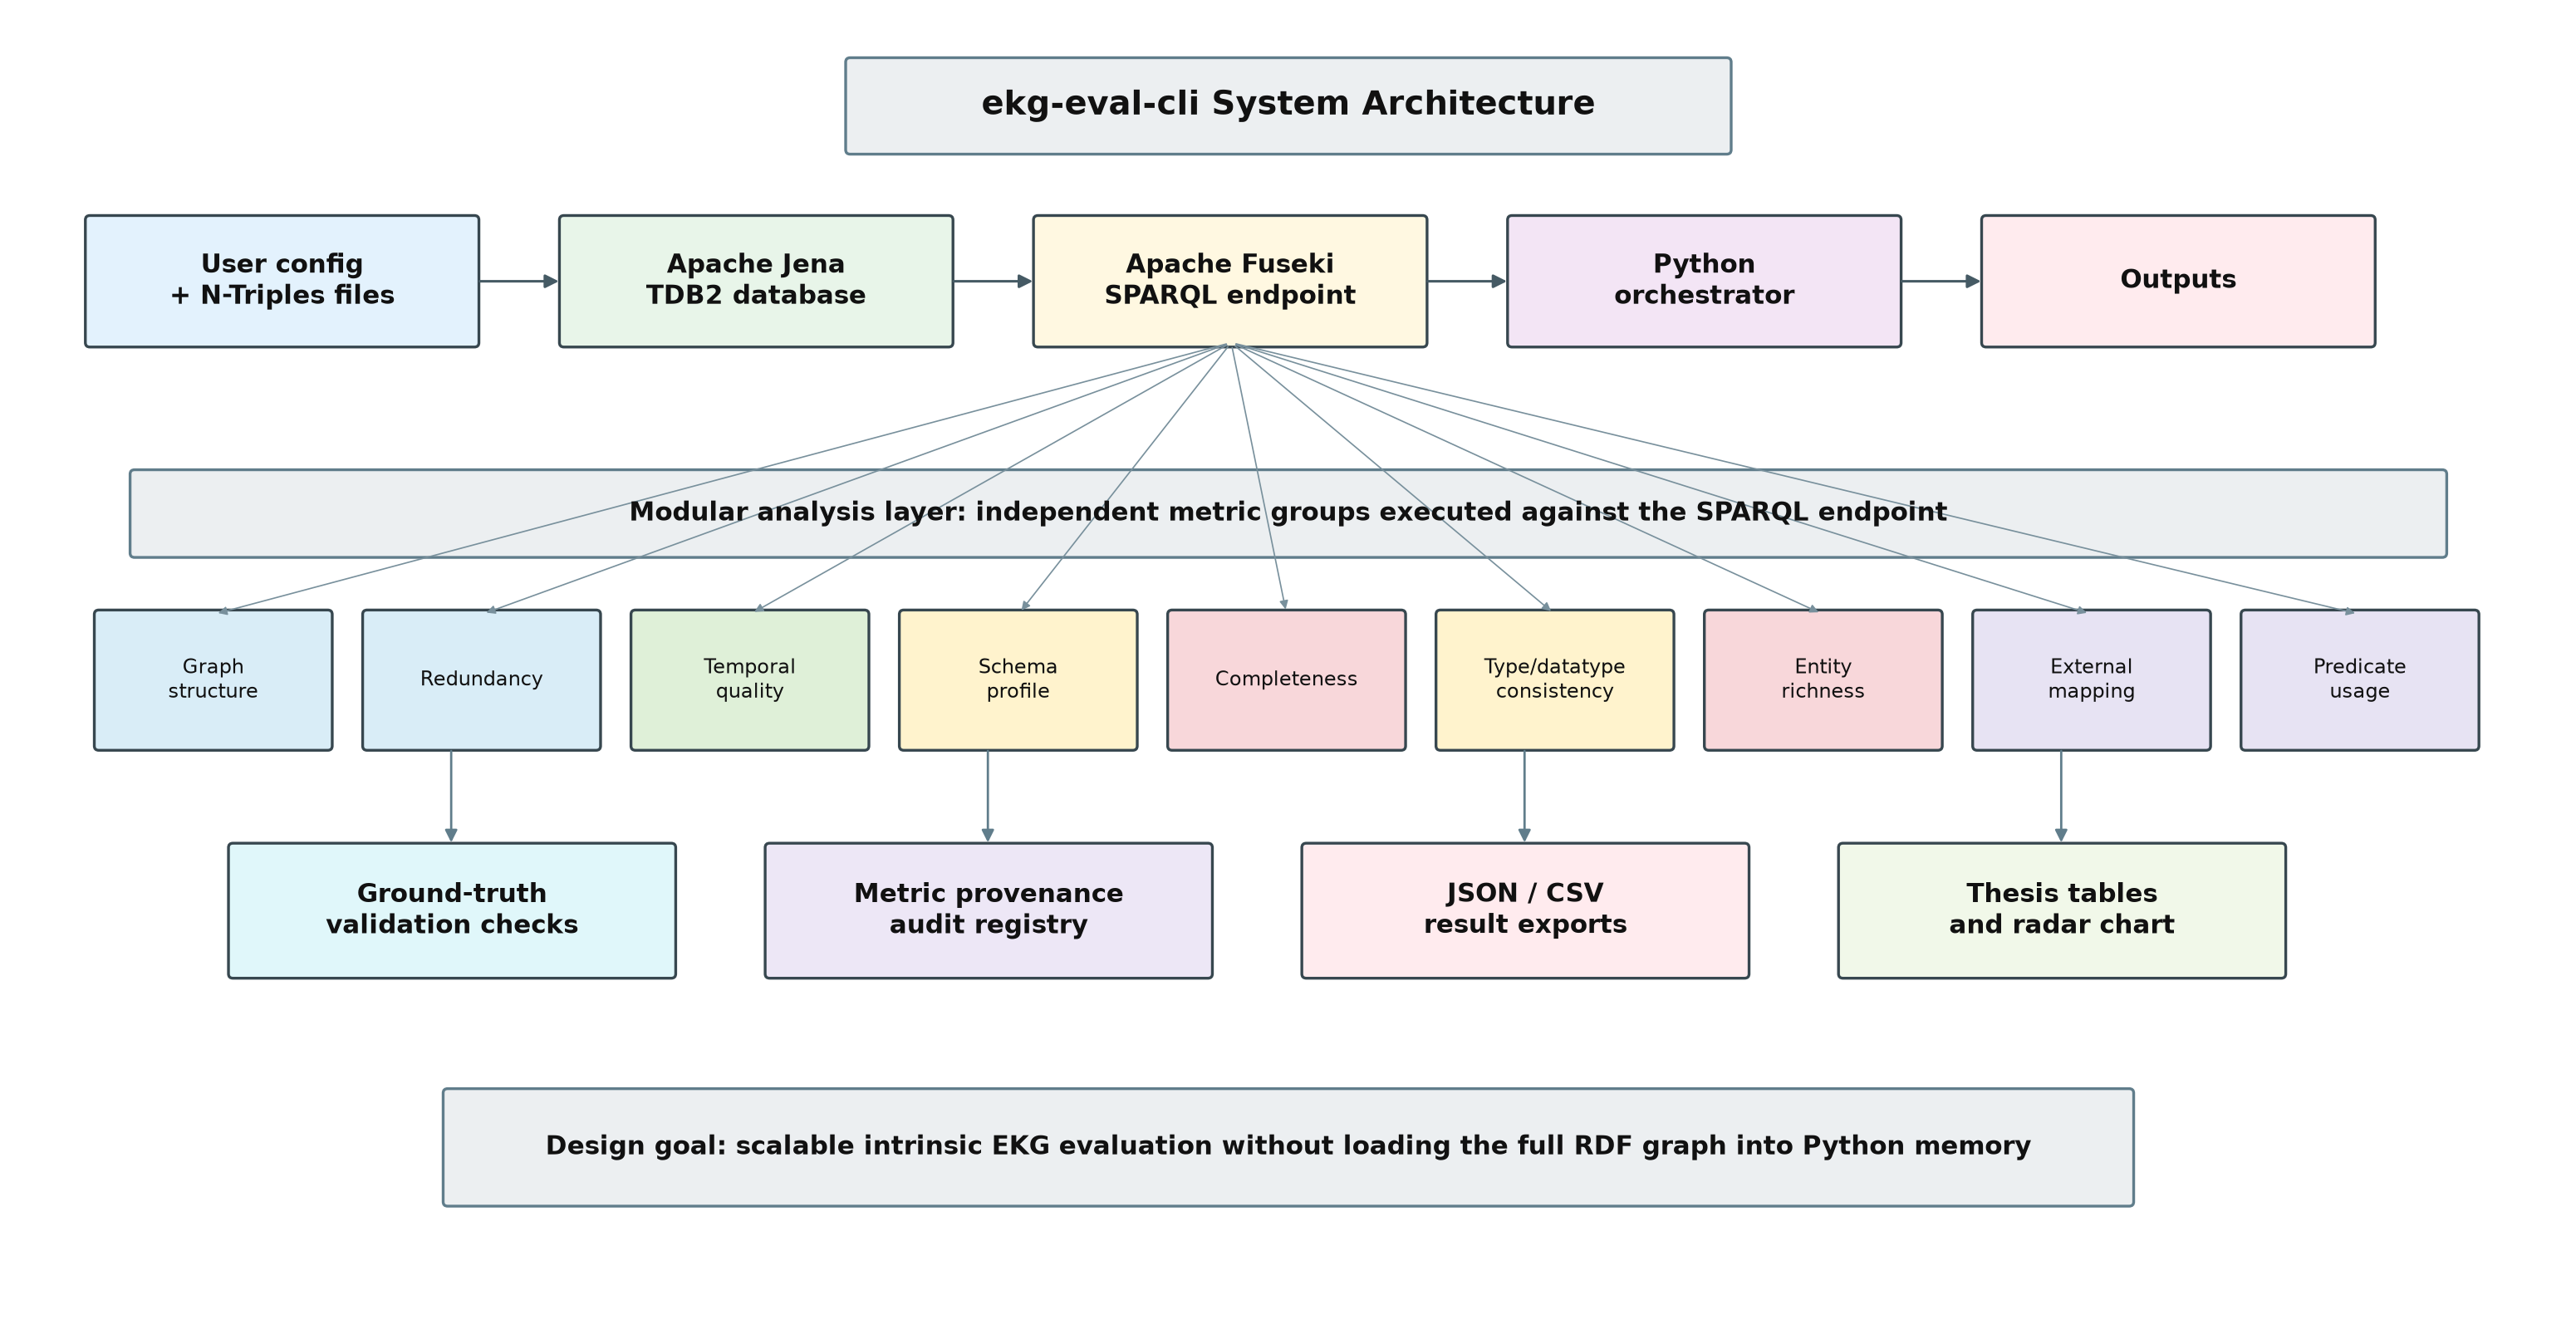
\includegraphics[width=\textwidth]{architecture.png}
\caption{System architecture of the implemented evaluation pipeline, showing how user configuration and RDF inputs flow through Jena/Fuseki infrastructure, Python orchestration, modular analysers, verification checks, and reporting outputs.}
\label{fig:architecture}
\end{figure}

\subsection{Technology Stack}

The implementation combines established semantic web infrastructure for RDF storage and querying with Python-based libraries for graph analysis and data processing. Apache Jena and Fuseki were chosen as the RDF backend because they are widely used open-source semantic web tools for RDF storage and SPARQL access, supporting compatibility with standard RDF EKG inputs. Python was selected as the implementation language for its rich ecosystem of data analysis libraries. Table \ref{tab:techstack} summarises the technology stack.

\begin{table}[h]
\centering
\caption{Technology stack}
\label{tab:techstack}
\begin{tabularx}{\textwidth}{llX}
\toprule
\textbf{Technology} & \textbf{Version} & \textbf{Role} \\
\midrule
Apache Jena & 5.6.0 & RDF triple store (TDB2) for storage and indexing \\
Apache Fuseki & 5.6.0 & SPARQL 1.1 server providing HTTP query endpoint \\
Python & 3.12.6 & Implementation language used for the final runs \\
NetworkX & 3.3 & In-memory graph connectivity and structural metrics \\
Click & 8.1.7 & Command-line interface framework \\
RDFLib & 7.6.0 & RDF parsing utilities for data validation \\
RapidFuzz & 3.14.5 & Deterministic fuzzy string comparison \\
DuckDB & 1.5.5 & Disk-backed edge storage and deduplication in large-graph mode \\
NumPy/Numba & 1.26.4/0.66.0 & Array-backed union-find for large graph projections \\
\bottomrule
\end{tabularx}
\end{table}
\clearpage

\subsection{Key Design Decisions}

Several design decisions shaped the implementation. Semantic metrics are queried through SPARQL, while exact file scans are used for selected profile counts on very large inputs; neither route loads the complete OEKG graph into Python memory. Structural analysis uses the domain projection defined above. TDB2 and large-graph artefacts are reused only when their manifests match the input hashes and relevant projection contract. Each dimension has an independent analyser but shares the same list of result definitions and population rules. Fuzzy matching always uses RapidFuzz exact all-pairs comparison inside the deterministic bounded sample, so installing an optional package cannot change the algorithm.

\subsection{Settings That Affect the Results}

The same settings must be used when results are compared. Each result file therefore records the similarity threshold, sample sizes, type-alignment limit, and namespace allow-list. The accepted runs use a 0.90 fuzzy-label threshold, the first 1,000 eligible event labels for fuzzy comparison, 1,000 temporal values or events, and at most 50 declared properties for type alignment. Label uniqueness uses the first 5,000 eligible events, and the non-allowlisted-property report shows at most 50 predicates. Table \ref{tab:default_parameters} records these settings and the standard namespaces included in the allow-list.

\section{Reproducing the Evaluation}

The repository provides one entry point for reproducing the evaluation: \url{https://github.com/tadiwa-aizen/ekg}. After cloning it, the recommended examiner command from the \texttt{ekg} folder is:

\begin{verbatim}
.\reproduce.ps1 -Mode Quick
\end{verbatim}

\texttt{Quick} creates a locked environment, runs the 24 automated tests, regenerates D1--D3, evaluates them, and checks all 32 registered fields against the accepted evidence. \texttt{Verify} only checks the stored source, input, result, test, comparator, and figure records. \texttt{Full} also reruns the three ChronoGrapher artefacts and the complete cleaned OEKG event layer and therefore needs substantially more time and disk space. Each mode writes a new report folder and does not overwrite the accepted evidence. Exact commands, expected outputs, data preparation, and storage requirements are documented in \texttt{ekg/REPRODUCE.md} and Appendix A.

The accepted evaluation was checked again using \texttt{Verify} and \texttt{Quick}. The integrity check passed all 20 stored-evidence checks. The fresh quick run passed all 24 automated tests and reproduced all 32 registered D1--D3 fields exactly.

\subsection{Recorded Evaluation Settings}

The default parameters used for the reported results are summarised in Table \ref{tab:default_parameters}. The result files record these values together with the input files, software version, and output status needed to interpret the run.

\begin{table}[H]
\centering
\caption{Default evaluation parameters used for the reported results}
\label{tab:default_parameters}
\begin{tabularx}{\textwidth}{lX}
\toprule
\textbf{Parameter} & \textbf{Default value and role} \\
\midrule
Fuzzy similarity threshold & 0.90, applied to exact RapidFuzz token-sort comparisons within the disclosed sample. \\
Fuzzy matching sample size & First 1,000 eligible events ordered by event IRI; no population estimate is made. \\
Label-uniqueness reporting limit & First 5,000 eligible events ordered by event IRI; fixed in the final implementation. \\
Temporal validation sample size & 1,000 values or events selected by the recorded deterministic procedure. \\
Type-alignment property limit & First 50 declared properties ordered by property/domain/range IRI. \\
Non-allowlisted-property reporting limit & Up to the 50 most frequent distinct predicates outside the allow-list; fixed in the final implementation. \\
Standard namespace allow-list & RDF, RDFS, OWL, XSD, SEM, Schema.org, EventKG schema, FOAF, SKOS, Dublin Core, DBpedia ontology, and Wikidata entity namespaces. \\
\bottomrule
\end{tabularx}
\end{table}

\subsection{How the Implementation Was Checked}
\label{sec:validation}

The checks answer a specific question: does the implementation return the values defined by the framework? The final suite uses small RDF fixtures whose expected answers can be calculated by hand. Together, the fixtures cover all 32 registered fields, including empty or inapplicable cases, graph projection, label normalisation, temporal ordering, type applicability, mapping hosts, and predicate-distribution formulae. Selected totals were also compared with the input files and direct SPARQL queries. Passing these checks shows that the program follows its declared calculation rules for the fixtures; it does not prove that every metric is suitable for every EKG. Appendix A records the exact command and environment.

Input compatibility was checked separately. The default profile expects direct \texttt{sem:Event} assertions and SEM timestamps attached to those events. A graph using another vocabulary or storing time on relation nodes needs a declared mapping before the affected metrics can be interpreted. If the required evidence does not exist, the evaluator reports \texttt{N/A} and the relevant counts rather than a perfect score.

\subsection{How the External Tools Were Compared}

RDFUnit, KGHeartBeat, Luzzu, and SANSA were given the same 16 N-Triples files for each of D1--D3. Their input records were checked against those used by the proposed evaluator. The comparison asks two questions: which selected EKG dimensions each tool covers, and whether its own outputs change across D1--D3. Values are compared only within the same tool and metric because the tools use different definitions and scales. The repository retains a frozen summary of the input hashes, tool revisions, local patch hashes, native values, and failures. Appendix \ref{app:comparator_reproducibility} records the execution boundary and the local adaptations.

\section{Datasets and Study Context}

The empirical study combines controlled synthetic data, general-tool baselines, and independently produced RDF event graphs. These sources serve different purposes: sensitivity testing, comparison with narrower evaluators, and real-world feasibility assessment.

\subsection{Synthetic Datasets}

Three synthetic EventKG-style datasets were created for controlled sensitivity testing. Synthetic data were chosen because declared generation parameters provide known perturbations, the changes can be reproduced, and metric responses can be inspected without relying on inaccessible annotations. This is not an independent accuracy benchmark: the profiles were designed around properties that the framework measures. External feasibility is assessed separately through the OEKG and ChronoGrapher runs.

Dataset 1, \texttt{synthetic-event-kg}, is the high-quality baseline with 100 direct events. It was generated with high quality by construction: every direct event has temporal information, event labels are unique, external links are complete, and event descriptions are comparatively rich. It establishes the upper controlled profile, not factual ground truth.

Dataset 2, \texttt{synthetic-event-kg-2}, is the mixed-quality dataset with 120 direct events. It uses the same file structure and ontology as Dataset 1 but intentionally introduces partial degradation, including lower label uniqueness, reduced temporal coverage, lower minimum-profile completeness, weaker external-link coverage, and less descriptive event records. It tests whether the framework detects a middle profile rather than only separating clean and poor data.

Dataset 3, \texttt{synthetic-event-kg-3}, is the low-quality dataset with 120 core events. It remains a structurally valid EKG but is intentionally degraded across most informative dimensions: low label uniqueness, low temporal coverage, coarser temporal granularity, low external-link coverage, low population completeness, and many sparse event descriptions. It tests whether the framework can detect broad degradation and distinguish the low-quality profile from D1 and D2.

All synthetic datasets follow the Simple Event Model (SEM) ontology and use standard RDF/RDFS/OWL vocabularies. Events include temporal anchors, participants, places, labels, descriptions, and external links using \texttt{owl:sameAs} to Wikidata and DBpedia-style resources. The final datasets were generated by a single deterministic script, \texttt{create\_tiered\_synthetic\_eventkgs.py}, rather than separate hand-edited files. The script uses controlled profile parameters for event count, text-event count, entity count, label coverage, date coverage, place coverage, external-link coverage, description coverage, relation density, unique-label pools, and temporal granularity. This makes the intended high-, mixed-, and low-quality profile differences explicit by construction while keeping the same EventKG-style file layout across datasets; it does not require every descriptive metric to form a strict total ordering.

All event-level coverage, completeness, redundancy, temporal, richness, mapping, and type-alignment rates use direct \texttt{sem:Event} resources as their event population, comprising 100 events in D1 and 120 in D2 and D3. Graph-structure metrics instead use the declared domain-relation projection, and predicate-distribution metrics use the RDF predicate-frequency distribution. Generated text-event resources and subclass diagnostics remain supporting context and are not substituted into a direct-event numerator or denominator. This prevents the population inconsistency identified in earlier completeness results while retaining the appropriate unit for graph-level metrics.

Each generated dataset contains 16 N-Triples files and three Turtle files: event files, entity files, relation files, type files, label files, description files, property-label files, DBpedia-type ontology files, \texttt{schema.nt}, \texttt{schema.ttl}, \texttt{void.ttl}, and \texttt{graphs.ttl}. The schema and file layout were kept stable across all three datasets so that quality differences arise from controlled data-profile changes rather than from incompatible input formats.

\subsubsection{Synthetic Dataset Construction Procedure}

The datasets were constructed through a deterministic generation procedure rather than by manually editing RDF files. The generator first defines three profile objects, one for each intended quality level. Each profile specifies the number of core events, text events, and entities to create, together with probability parameters controlling whether an event receives a label, date, place, external link, description, and event-entity relation. A fixed random seed based on the profile's event-prefix value is then used so that the same script produces the same RDF files on repeated runs.

For each profile, the generator clears the previous output files and writes a complete EventKG-style folder. It first creates event resources typed as \texttt{sem:Event}, optionally adding English labels and \texttt{owl:sameAs} links to Wikidata and DBpedia-style resources according to the profile's label and external-link rates. It then writes event temporal and place relations, using \texttt{sem:hasBeginTimeStamp}, \texttt{ekgs:startUnitType}, and \texttt{sem:hasPlace}. Dataset 2 introduces some year-only dates, while Dataset 3 introduces both year-only dates and clustered dates, so temporal degradation affects not only coverage but also granularity and distribution.

The generator next creates event-entity relation nodes, literal descriptions, entity resources, text-event resources, entity-entity relations, type assertions, preferred labels, first-sentence descriptions, property labels, and small ontology-support files. The same RDF file names are used for all three datasets. This matters methodologically because the evaluation tool sees the same input structure in every case; only the controlled quality properties differ.

The benchmark-support files used for the poster-stage comparison are separate from the graph datasets. Files such as Event-QA-style queries, EventKG-style coverage profiles, and other comparison artefacts were stored in support folders and were not treated as additional graph content for the core thesis evaluation. The clean deliverable datasets therefore contain only the RDF source files needed to load and evaluate the three graph profiles.

Table \ref{tab:synthetic_generation_profile} records the principal parameters used by the deterministic generator.

\begin{table}[H]
\centering
\caption{Controlled generation profile for the three synthetic datasets}
\label{tab:synthetic_generation_profile}
\scriptsize
\begin{tabular}{lccc}
\toprule
Generation parameter & Dataset 1 & Dataset 2 & Dataset 3 \\
\midrule
Core events & 100 & 120 & 120 \\
Text events & 40 & 35 & 25 \\
Entities & 320 & 180 & 80 \\
Label rate & 1.00 & 0.75 & 0.45 \\
Date rate & 1.00 & 0.70 & 0.40 \\
Place rate & 0.95 & 0.55 & 0.10 \\
External-link rate & 1.00 & 0.60 & 0.12 \\
Description rate & 0.90 & 0.50 & 0.10 \\
Relation coverage & 0.95 & 0.65 & 0.20 \\
Unique-label pool & 100 & 55 & 8 \\
Temporal degradation & None & Some year-only dates & Clustered, coarse dates \\
\bottomrule
\end{tabular}
\end{table}

\subsection{Real-World Datasets}

\textbf{OEKG event-layer dataset:} The production-scale feasibility evaluation uses OEKG, specifically the published OEKG event layer. OEKG is an integrated open event knowledge graph designed around event-centric integration and cross-lingual use cases \citep{oekg2023}. The local input used for this thesis consisted of 13 N-Triples files covering event resources, event labels, event descriptions, temporal and place relations, event relation nodes, type assertions, schema triples, and DBpedia type-label support. The run therefore tests execution on real published OEKG event data rather than only on synthetic data.

The real dataset was loaded into an Apache Jena TDB2 database and exposed through Fuseki for RDF-native metrics. Cleaning was deliberately minimal. The preparation script copied the selected event-layer files into a separate working folder, leaving most files unchanged. Only invalid backslash escapes inside string literals were repaired so that Apache Jena could parse the N-Triples input; this changed seven lines in \texttt{relations\_events\_literals.nt}. No new event facts were added, no quality values were edited, and the original extracted OEKG archive was left unchanged. The resulting TDB2 database contained 954,554 direct \texttt{sem:Event} records. This dataset is substantially larger than the synthetic datasets and is used to test whether the framework can produce a reproducible quality profile on a real EKG under local workstation constraints.

This dataset should be interpreted as OEKG's event layer rather than as every file in the full OEKG distribution. This distinction matters because the OEKG paper describes a graph of more than 400 million triples integrated from seven datasets, including event knowledge, question answering resources, recommendation traces, images, news articles, and named-entity resources \citep{oekg2023}. The selected event layer is the relevant feasibility target for this thesis because it contains the core RDF event resources, event labels, temporal and place relations, type assertions, and external links on which the implemented intrinsic EKG metrics operate. It therefore supports a production-scale feasibility claim for OEKG event data, but not a claim that every non-event support graph in the complete OEKG archive has been evaluated. Full preparation details are given in Appendix \ref{app:oekg_run_details}.

\textbf{ChronoGrapher public RDF graph artefacts:} A second real-world feasibility evaluation used the public RDF/Turtle graph artefacts released with ChronoGrapher, an event-centric knowledge graph construction approach based on informed graph traversal \citep{chronographer2023}. Three graph artefacts were evaluated: \texttt{eventkg\_ng}, \texttt{search\_ng}, and \texttt{generation\_ng}. These files contain explicit \texttt{sem:Event} resources and SEM-style temporal and contextual properties. A fourth file, \texttt{frame\_ng}, was inspected but excluded from EKG evaluation because it did not contain explicit \texttt{sem:Event} type assertions.

The ChronoGrapher files were validated as Turtle and converted to UTF-8 N-Triples before evaluation. Unlike the OEKG event-layer dataset, these artefacts are small experimental graphs rather than a production-scale published event layer. Their value in this study is therefore different: they test whether the framework can run on an independently produced public RDF event-graph artefact and whether it can expose intrinsic quality properties that were not the main focus of the original ChronoGrapher construction and question-answering evaluation. The results are interpreted with this boundary: low scores on labels, explicit external mappings, or minimal profile conformance indicate mismatch with the thesis's EventKG-style intrinsic profile assumptions, not a general claim that ChronoGrapher is low quality for its original task.

\subsubsection{Large-Graph Execution Mode}

The original implementation used NetworkX for graph-structure metrics after projecting RDF IRI-to-IRI triples into an undirected graph. This was suitable for the synthetic datasets but was not feasible for the OEKG event layer on the available machine. The projected OEKG event-layer graph contained tens of millions of edges, and a NetworkX attempt ran for several hours without producing results while consuming substantial memory.

To complete the real-graph evaluation within the available hardware, the implementation was extended with a \texttt{--large-graph-mode}. In this mode, RDF-native metrics still use Jena/Fuseki or exact N-Triples file scans, but graph-structure metrics are computed without materialising the full projected graph in NetworkX. The large-graph path streams N-Triples files, keeps only IRI-to-IRI triples, removes self-loops, canonicalises each edge as an undirected pair, and stores the projection in DuckDB. DuckDB is then used to deduplicate edges and assign dense integer node identifiers. Connected components are computed by streaming the integer edge table through a union-find data structure backed by NumPy arrays.

This produces exact values for projected node count, edge count, average degree, density, connected components, and giant component size/ratio under the declared simple undirected IRI projection. Edge connectivity is reported conditionally: because the OEKG projected graph is disconnected, global edge connectivity is exactly 0. Average clustering is not computed in large-graph mode and is explicitly reported as unavailable. This limitation is retained in the results rather than hidden.

\subsection{Dataset Characteristics}

Table \ref{tab:datasets} summarises the characteristics of evaluation datasets.

\begin{table}[H]
\centering
\caption{Evaluation dataset characteristics}
\label{tab:datasets}
\begin{tabular}{>{\raggedright\arraybackslash}p{3.4cm}>{\raggedright\arraybackslash}p{3.2cm}>{\raggedright\arraybackslash}p{2.2cm}>{\raggedright\arraybackslash}p{3.2cm}}
\toprule
\textbf{Dataset} & \textbf{Core events} & \textbf{Quality profile} & \textbf{Purpose} \\
\midrule
synthetic-event-kg & 100 & High & Baseline \\
synthetic-event-kg-2 & 120 & Mixed & Sensitivity \\
synthetic-event-kg-3 & 120 & Low & Gradient \\
OEKG event layer & 954,554 direct \texttt{sem:Event} records & Real & Production-scale feasibility \\
ChronoGrapher \texttt{eventkg\_ng} & 235 & Real/public artefact & Independent RDF event-graph feasibility \\
ChronoGrapher \texttt{search\_ng} & 380 & Real/public artefact & Search-output quality profile \\
ChronoGrapher \texttt{generation\_ng} & 374 & Real/public artefact & Generated-graph quality profile \\
\bottomrule
\end{tabular}
\end{table}

\section{How the Framework Was Evaluated}

This section explains how the framework evaluation was organised before the results are reported in Chapter 4. The purpose was not to optimise an EKG for a single downstream task, such as question answering or event GraphRAG, but to test whether the framework can compute its intrinsic quality metrics correctly and use those metrics to reveal differences between EKGs.

The empirical assessment had four parts. First, implementation checks compared outputs with small RDF examples whose correct answers could be calculated by hand, as described in Section \ref{sec:validation}. Second, sensitivity analysis applied the framework to three controlled high-, mixed-, and low-quality profiles. Third, RDFUnit, KGHeartBeat, Luzzu, and SANSA were run on byte-identical copies of those inputs to compare their native coverage and response without constructing a common score. Fourth, real-world feasibility was tested on the complete cleaned OEKG event layer and the public ChronoGrapher RDF graph artefacts. Chapter 4 reports the results and the limits of each part.

\section{Ethical Considerations}

This research uses synthetic data and publicly released OEKG and ChronoGrapher RDF graph artefacts for technical evaluation. The synthetic datasets were generated programmatically and do not contain real personal information. The public RDF artefacts were used as research datasets with attribution to their original sources; any redistribution of third-party data should follow the licence terms stated by those sources.

The evaluation implementation is licensed under the MIT licence and included with the research artefacts. Its design decisions, algorithms, and verification procedures are documented to enable critical evaluation and extension by other researchers.

No human subjects were involved in this research. Implementation verification relied on automated assertions against hand-computable RDF fixtures and independently calculated expected values.

The research adheres to academic integrity principles through proper citation of prior work, transparent reporting of limitations, and honest disclosure of validation discrepancies discovered during metric verification.

\section{Chapter Summary}

This chapter described the methodology used to design, formalise, implement, and evaluate an intrinsic framework across nine selected dimensions for RDF-based event-centric knowledge graphs. It explained how the nine dimensions and 28 distinct calculations were selected and formalised, why the implementation exposes 32 result fields, and how those fields were checked.

The evaluation design uses three synthetic EventKG-style datasets, the OEKG event layer, and three public ChronoGrapher RDF graph artefacts. Implementation correctness is checked with small RDF examples whose answers can be calculated by hand, file-level counting, direct database queries, and comparisons between related results. For OEKG, the methodology also uses a large-graph execution mode to avoid loading the full projected graph into memory.

The next chapter presents the results of applying the framework to three synthetic datasets, the OEKG event-layer dataset, and ChronoGrapher public RDF graph artefacts, demonstrating its ability to detect quality differences across a controlled spectrum and to run on real published RDF event-graph data.

